\newpage
\chapter{Counter flow flames}
\section{Introduction}
The counter flame model in Camflow is a transient model capable of predicting the species profiles, velocity profile, and the temperature profile.  When the temperature profile is obtained from experiment, the model can be used to simulate only the species profiles and velocity profile by providing the experimentally observed temperature profile. In this case only the species transport equations,  momentum and continuity equations are solved. An initial guess of intermediate species needs to be provided. If the temperature profile is not known, the model can predict the temperature profile by solving the energy equation. In this case in addition to the intermediate species composition, an initial guess for the temperature profile also needs to be provided. 

\section{Fundamentals}
The equation of continuity in cylindrical coordinate by considering only axial and radial coordinate can be written as
\begin{equation}
 \frac{\partial \rho}{\partial t} + \frac{1}{r}\frac{\partial}{\partial r}(\rho rv) + \frac{\partial}{\partial z}(\rho u) = 0;
\end{equation}
The radial and axial momentum follows as
\begin{equation}
 \rho \bigg( 
 \frac{\partial v}{\partial t} +
 v\frac{\partial v}{\partial r}+
 u\frac{\partial v}{\partial x} \bigg) = -\frac{\partial p}{\partial r} +
\mu \bigg[\frac{\partial}{\partial r}\bigg(\frac{1}{r}\frac{\partial}{\partial r}(rv)\bigg) + \frac{\partial^2v}{\partial x^2}\bigg],
\end{equation}

\begin{equation}
 \rho \bigg( 
 \frac{\partial u}{\partial t} +
 v\frac{\partial u}{\partial r}+
 u\frac{\partial u}{\partial x} \bigg) = -\frac{\partial p}{\partial r} +
\mu \bigg[\frac{1}{r} \frac{\partial}{\partial r}\bigg(r\frac{\partial u}{\partial r}\bigg) + \frac{\partial^2u}{\partial x^2}\bigg],
\end{equation}
Assuming similarity near the center line, the axial velocity, radial velocity, temperature and species mass fraction turns out to be functions of time and axial coordinate. Defining v/r =V(x), and by applying boundary layer theory in the axial direction the continuity and momentum simplified to

\begin{equation}
\frac{\partial \rho}{\partial t} + \frac{\partial (\rho u)}{\partial x} + 2\rho V = 0
\end{equation}
\begin{equation}
 \rho \frac{\partial V}{\partial t} + \rho u \frac{\partial V}{\partial x} + \rho V^2 = -\Lambda + \frac{\partial }{\partial x}\bigg(\mu \frac{\partial V}{\partial x} \bigg),
\end{equation}
and
\begin{equation}
 \frac{\partial p}{\partial x} = 0.
\end{equation}
The eigen value $\Lambda$ of the system has to be solved with other dependent variables
\begin{equation}
 \frac{1}{r}\frac{\partial p}{\partial r} = \Lambda
\end{equation}
The energy equation is written as
\begin{equation}
 \rho c_p \frac{\partial T}{\partial t}+ \rho u c_p \frac{\partial T}{\partial z} - \frac{\partial }{\partial z}\bigg(\lambda \frac{\partial T}{\partial z} \bigg) + \frac{\partial}{\partial z} \sum_k j_k h_{k}  + \sum_k h_k\dot{\omega}_k = 0
\label{energy}
\end{equation}
and the species transport equation
\begin{equation}
 \rho \frac{\partial Y_k}{\partial t}+ \rho u \frac{\partial Y_k}{\partial z} + \frac{\partial j_k}{\partial z} = \dot{\omega}_k W_k, \quad k=1\ldots K_g
\label{species}
\end{equation}
with $j_k$ defined as
\begin{equation}
 j_k = -\rho D_{km} \frac{dY_k}{dz},
\end{equation}
The boundary conditions for the above system of equations are 
\begin{eqnarray}
 x = 0: \quad u=u_f(t), \quad V = V_f(t) \quad T=T_f(t), \quad Y_k = Y_{kf} \nonumber \\
x=L: \quad u=u_o(t), \quad V=V_o(t), \quad T=T_o(t), \quad Y_k = Y_{ko}
\end{eqnarray}
In the above equations, $\rho$ is the density in kg/m$^3$, $u$ is the axial velocity in m/s, $v$ is the radial velocity in m/s,  $Y_k$ is the mass fraction of the k\'th chemical species, $j_k$ the mass flux of the k\'the species in kg/$m^2-s$, $\dot{\omega}_k$ the molar production rate of the k\'the species in mol/m$^3$-s, D$_{km}$ the diffusion coefficient of the k\'the species in the mixture, $h_k$ the specific enthalpy in J/kg, and the $t$ the time in $s$.

\section{Input file}
An example of ``camflow.xml'' input file is shown below
{\scriptsize{

\begin{verbatim}
 <?xml version="1.0" encoding="ISO-8859-1"?>
<camflow>
   <reactor model="counterflow">    
    <length unit="cm">2</length>
  </reactor>
  <op_condition>
     <temperature>adiabatic</temperature>
     <twall unit="K">1073</twall>
     <pressure unit="bar">1</pressure>
     <strain>10</strain>
  </op_condition>
  <inlet>
     <fuel>
       <velocity unit="m/s">1.0</velocity>
       <temperature unit="K">300.0</temperature>
       <molefrac>
        <species name="H2">1.0</species>
       </molefrac>
     </fuel>
     <oxidizer>
       <velocity unit="m/s">1.0</velocity>
       <temperature unit="K">300.0</temperature>
       <molefrac>
        <species name="O2">0.21</species>
        <species name="N2">*</species>
       </molefrac>
     </oxidizer>
  </inlet>
  <solver mode="coupled" solver="cvode" residual="on">
     <maxTime>10000</maxTime>
     <iterations>10</iterations>
     <tols>
        <resTol>1</resTol>
        <species>
           <aTol>1.e-12</aTol>
           <rTol>1.e-08</rTol>
        </species>
        <temperature>
           <aTol>1.e-03</aTol>
           <rTol>1.e-03</rTol>
        </temperature>
        <flow>
           <aTol>1.e-03</aTol>
           <rTol>1.e-03</rTol>
        </flow>
     </tols>
  </solver>
  <initialize>
    <mCenter unit="cm">1</mCenter>
    <mWidth unit="cm">0.5</mWidth>
    <massfrac>
      <intrmdt name="H">0.1</intrmdt>
      <intrmdt name="OH">0.12</intrmdt>
      <intrmdt name="HO2">0.001</intrmdt>
      <intrmdt name="H2O">0.01</intrmdt>
    </massfrac>
    <Tprofile unit_L="cm" unit_T="K">
      <position x="0.00">300.0</position>
      <position x="0.10">301.3</position>
      <position x="0.14">304.5</position>
      <position x="0.17">313.6</position>
      <position x="0.31">579.5</position>
      <position x="0.38">887.8</position>
      <position x="0.63">2221.0</position>
      <position x="0.66">2290.0</position>
      <position x="0.73">2019.0</position>
      <position x="0.75">1850.0</position>
      <position x="0.81">954.0</position>
      <position x="0.82">729.8</position>
      <position x="0.86">370.9</position>
      <position x="0.88">325.4</position>
      <position x="0.95">300.4</position>
      <position x="0.97">300.1</position>
      <position x="1.10">300.0</position>
      <position x="1.18">300.0</position>
      <position x="1.75">300.0</position>
      <position x="1.95">300.0</position>
      <position x="2.00">300.0</position>
    </Tprofile>
 </initialize>
 <report outfile="final" species="mole">
 </report>
 <grid>grid.inp</grid>
</camflow>

\end{verbatim}}
}

The input file follows xml standard. A detailed description about the various elements in the input file is specified below.

\begin{itemize}
 \item \textbf{rector} : The reactor element specifies which model is to be simulated and for a counter flow flame camflow expects ``counterflow'' as the model attribute value. The reactor element also holds child element length for specifying the nozzle separation, and is given with the unit attribute. The unit of the value specified can be in ``cm'', ``m'', or in ``in''ches. Appropriate attribute must be specified. However,, the grid file (described later) has higher precedence over the value specified here.

\item \textbf{op\_conditions} : The element op\_conditions describes the operating conditions for the flame. This includes the specification of the pressure and the condition applied to the solution of energy equation. The flame pressure may be specified in the units of ``Pa'', ``atm'', or ``bar''. The temperature element can take the values of ``isothermal'', ``adiabatic'', or ``userdefined''. In the case of isothermal calculation, the energy equation is not solved and the flame is assumed to be at the same temperature as the incoming fuel. The user may also perform the integration for a pre-calculated or measured temperature profile. In this case the temperature child element must be assigned with the value ``userdefined'' and the user defined temperature profile can be specified (explained later). For adiabatic calculations, provide the temperature element with the value ``adiabatic'', and in this case the energy equation will be solved to predict the temperature profile.\\

In addition to the temperature and pressure, the strain rate needs to be specified since camflow does not solve for the pressure gradient eigen value. Instead it is calculated from the strain rate according to
\begin{equation}
 \Lambda = -\rho_o a^2
\end{equation}

\item \textbf{inlet} : For counter flow flames there are two inlets; one for the fuel and the other for the oxidizer. All properties pertaining to the fuel inlet must be specified under the element ``fuel'' and all properties pertaining to the oxidizer inlet must be specified under the ``oxidizer'' element. Both ``fuel'' and ``oxidizer'' element must specify the velocity at the inlet using the ``velocity'' element, temperature using the ``temperature'' element and the species composition using ``molefrac'' or ``massfrac'' element.The unit for velocity may be in m/s or in cm/s and temperature can be in C or in K. The appropriate units must be specified as attribute values. The chemical species present in the fuel/oxidizer can be specified using the species elements, with the species name as attribute and corresponding mole/mass fraction as attribute. The last species composition may be specified using ``*'', and this case the ``*'' will stand for 1-sum of composition of other species. 

\item \textbf{solver}: The solver element holds the solver control specifications. The attributes ``mode'' can be specified as ``coupled'' or ``segregated'' for counter flow flames. The solver name is essentially provided to switch from one solver to another. However, the present version of Camflow uses only CVode as the numerical integrator, and therefore accepts only ``cvode'' as the solver name. When the solver mode is specified as coupled, the governing equations are solved simultaneously, and for ``segregated'' mode, the governing equations are solved sequentially for a number of times that is specified by the element iterations. By default the value of iterations element is one. At the end of the number of iterations, the solution mode will automatically switch to coupled. The user is encouraged to use coupled mode for counter-flow calculations.\\

Additionally the integration time may be optionally specified by the element maxTime. By default the value of maxTime is 100000 s. However, the final integration time is the maxTime or the time required to reach steady state whichever is lower. This means the solver will stop integration, if steady state is reached before the specified integration time.\\

The element ``tols'' hold the various tolarences that can be applied to the species, energy, and continuity equations. For species a relative tolarence of at least 10$^{-6}$ should be used. The user may need to adjust the tolarence values for the species in case of solution difficulties.

\item \textbf{initialize} The initialize element can be used to specify various initial conditions. 
A guess value for the intermediate species composition may be used to initialize the flow filed. When specifying the intermediate compostions, the mixing center and mixing width needs to be specified. When these compositions are specified a guassien profile will be generated for the intermediate species with peaks at the mixing centers and the having the spread specified by mixing width. The mixing center is specified by the element ``mCenter`` and the mixing width is specified by ''mWidth``. Both these elements are provided with ''unit`` attribute, and appropriate unit of length must be specified. Unlike the specification of fuel inlet species composition, the sum of intermediate or product species composition need not to sum up to one. However, the user must ensure that the sum does not exceeds one.\\

The temperature profile can be specified by using the ``Tprofile'' element with two attributes namely ``unit\_L'' for length unit and ``unit\_T'' for temperature unit. The length unit can be in ``cm'' or in ``m'', where as the temperature unit can be either in ``K'' or in ``C''. The actual temperature as a function of reactor position is specified with the child elements position with the attribute ``x'', which stands for the position with the reactor. If the length unit is specified as ``cm'' then ``x'' is the position from the reactor inlet in ``cm'', and the value for the position element is the temperature at position ``x''.

\item \textbf{report}: The desired output for the species composition must be specified in this element using the species attribute. ``mole'' or ``mass'' may be used as the attribute values, and correspondingly the output will be produced either in mole fraction or mass fractions.

\item \textbf{grid}: The premix flame model requires a descretised geometry. The geometry may be specified using anyfile that contains a nodes of the descretised geometry. The content of the grid file is assumed to be in ``m'' units. An example is shown below\\
{\scriptsize{\begin{verbatim}
0.0
0.0002
0.0003
0.0004
0.0005
0.0006
0.0007
0.0009
0.001
0.0015
0.002
0.003
0.004
0.005
0.006
0.007
0.008
0.009
0.01
0.02
0.03
0.04
0.05
\end{verbatim}
}}

The content of the grid file has precedence over the length of the flame specified in the reactor element. This means that the length of the flame after reading the grid file will be set to the final point specified in the grid file.
\end{itemize}

\section{Executing the binary}
The counter flow flame model of Camflow expects four input files namely, ``camflow.xml'', ``therm.dat'',  ``chem.inp'', and ``tran.dat''. All the files must be present in the working directory. Upon succesful execution the output file ``profile.dat'' containing the final integration time (s), axial position (m), residence time (1/s), density (kg/m$^3$), velocity (m/s), massflow rate (kg/m$^2$s), temperature (K), and the species compositions in mass or mole fractions.

\section{Results}
The following figures shows the velocity profile (Fig.~\ref{velocity}), temperature profile (Fig.~\ref{temp}), and species profiles (Fig.~\ref{species_profile}) resulting from hydrogen oxygen flame with 100 \% H$_2$ on the fuel side and air on the oxidizer end.

\begin{figure*}[h]
 \centering
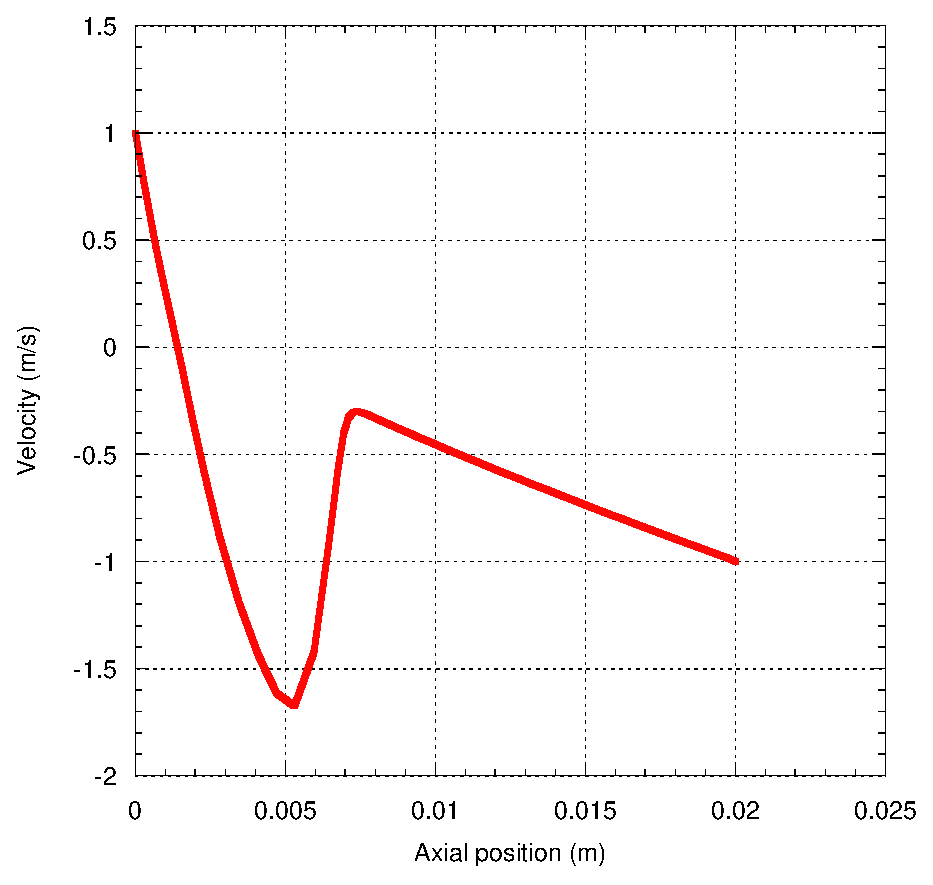
\includegraphics[scale=0.6]{velocity.eps}
\caption{Velocity profile for hydrogen flame}
\label{velocity}
\end{figure*}

\begin{figure*}[h]
 \centering
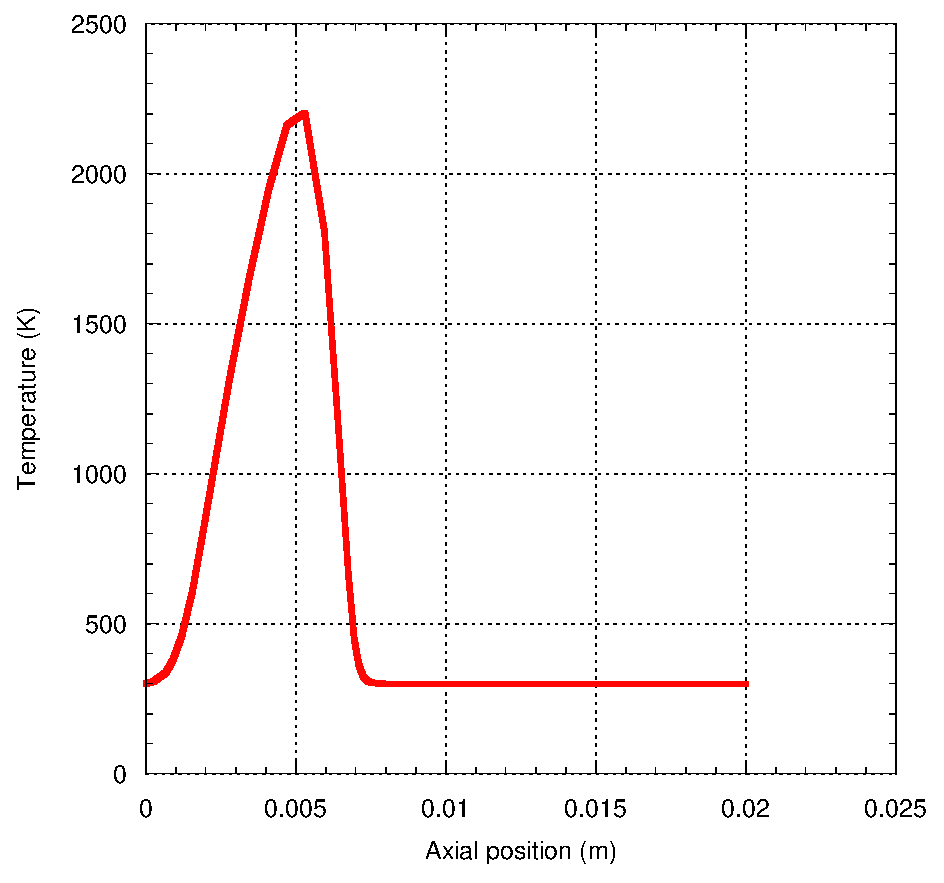
\includegraphics[scale=0.6]{temp.eps}
\caption{Temperature profile for hydrogen flame}
\label{temp}
\end{figure*}

\begin{figure*}[h]
 \centering
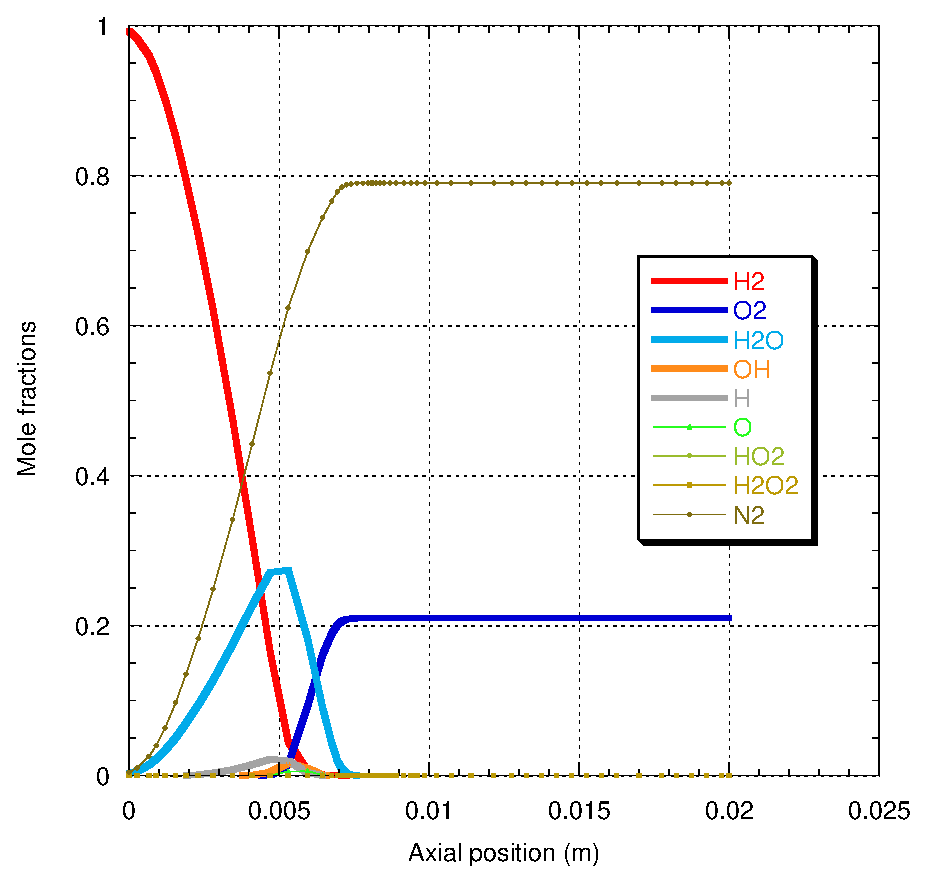
\includegraphics[scale=0.6]{counter_profile.eps}
\caption{Species profile for hydrogen flame}
\label{species_profile}
\end{figure*}

%===============================================================================================
%
%
%
%===============================================================================================
